\section{SmartElement}

SmartElement är ett back-end system som sköter filtrering av innehåll på basis av information som samlas in om besökare på en webbsida. Upprätthållare av en webbsida kan genom att integrera SmartElements JavaScript tag i sin sida, låta back-end systemet fylla i specicficerade element med personaliserat innehåll.

\subsection{Beståndsdelar}

\begin{figure}[h!]
\centering
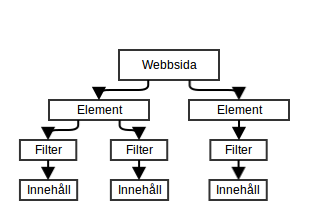
\includegraphics[width=120mm]{assets/images/smelementdatamodelabstract.png}
\caption{Exempel på en hierarki i SmartElement}
\label{abstractstructure}
\end{figure}

SmartElement bygger på några grundläggande koncept; webbsidor, element, filter och innehåll. Med dessa fyra byggstenar konfigureras det objekt, visualiserat i bild \ref{abstractstructure}, som back-end systemet använder för att filtrera och leverera innehåll.

\subsubsection{Webbsidan}

Webbsidan är det högsta elementet som SmartElement handskas med. Det representerar en hel webbplats, under vilken man kan definiera element och innehåll. Varje sida har en unik identifikationsnummer som används för att hämta ladda SmartElement tagen.

\subsubsection{Element}

Elementen är hållare för den data som returneras från back-end systemet och det som knyter innehållet till webbsidan. Elementet har i sig flere innehåll och filter, filtren används för att välja ut det innehåll som skall visas i elementet. Element har en inom sidan unik kod som används för att specificera vilka element som behöver processeras när man kallar på back-end systemet.

\subsubsection{Filter}

Filter berstår i SmartElement av flere olika regler som ställer en fråga om besökaren samt en länk till ett innehåll, vilket visas om filtret matchar. För att ett filter skall matcha krävs det att besökaren passar alla regler i filtret. För att hantera fall var två eller flere filter passar för en beökare har filter en prioritetsordning inom elementet, valbar av användaren.

\subsubsection{Innehåll}

Innehåll är den konkreta data som levereras för ett element efter att ett filter valts som vinnare. Innehållet kan bestå av text, HTML kod eller \gls{json} data, det är upp till användaren att definiera vad för data som sparas.